%! TeX program = lualatex
\documentclass[../main.tex]{subfiles}

\ifcsname preamble@file\endcsname
  \externaldocument[main-]{../../build/main}
  \setcounter{page}{\getpagerefnumber{main-week4}}
\fi

\begin{document} \makelectureweek{4}

\section{The tangent line of a curve}

\begin{example}
  A line \(L\) passes through the point \(P = (-1,\frac{3}{2})\) and has a slope of \(m = -\frac{1}{2}\). 
  \begin{enumerate}
    \item Write down the \emph{point-slope form} of the line \(L\).
      \vspace{2in}

    \item Write down the \emph{slope-intercept form} of the line \(L\).
      \vspace{2in}

    \item Draw \(L\).
  \end{enumerate}

  \begin{tikzpicture}
    \begin{axis}[
      axis equal,
      axis lines=center,
      grid=both,
      ymin=-1, ymax=3,
      xmin=-3, xmax=3,
      xlabel={\(x\)},
      ylabel={\(y\)},
      xlabel style={ at={(ticklabel* cs:1)}, font=\footnotesize, anchor=west  },
      ylabel style={ at={(ticklabel* cs:1)}, font=\footnotesize, anchor=south },
      yticklabel style={font=\footnotesize, /pgf/number format/.cd,frac},
      xticklabel style={font=\footnotesize, /pgf/number format/.cd,frac},
      ]
      % \addplot[blue,domain=-3:3] {-1/2*x + 1};
    \end{axis}
  \end{tikzpicture}

  \vfill
  \faBookReader{} Review page 22 for the point-slope form and page 141 for the slope-intercept form of a line.
\end{example}
\clearpage

% The line \(L\) is tangentially related to the fuction \(f(x)\) at the point \(P\).
\begin{mdframed}[style=withref]
  \textbf{Definition}. The \emph{tangent line to the curve \(y = f(x)\) through a point \(P = (a,f(a))\)} is the line through \(P\) with slope 
  \begin{equation} \label{eq:tangent1}
    m = \lim_{x \to a} \frac{f(x) - f(a)}{x - a}
  \end{equation}
  provided that this limit exists. The slope of the tangent line (at a point \(P\)) is also called the \emph{slope of the curve} (at the point \(P\)).
  
  \textbook{\stewart{141}{\fbox{1} Definition}}
\end{mdframed}
% the tangent line does not exists if you cannot calculate this limit.

\begin{example} \label{ex:cubic}
  Consider the curve \(y = x^{3}\) through the point \(P = (1,1)\).

  \begin{enumerate}
    \item Calculate the slope \(m\) of the tangent line at \(P\) from the definition if the tangent line exists.
      \vfill

    \item Write down the \emph{point-slope} form of the equation of the tangent line. Draw the tangent line on the graph below.

      \includegraphics{../standalones/build/plot_tangent_exercise}
  \end{enumerate}
\end{example}
\clearpage

We use Example~\ref{ex:cubic} to demonstrate why the slope of a curve is defined as \(m = \lim_{x \to a} \frac{f(x) - f(a)}{x - a}\).

% when we think about the slope of a straight line, we think about how fast it changes at a point.
% we want the slope of the curve to say mean exactly that --- how fast the it changes around P. 
% the slope should make sense for more general curves.
\includegraphics{../standalones/build/plot_tangent_exercise}
\bigskip


\begin{example}
  Study the curve \(y = |x|\) at the origin in two different ways.
  \begin{enumerate}
    \item Calculate the slope of the curve at the origin from the definition, if the slope exists. 
      \vfill

    \item Use the graph below to \emph{reason} if the tangent line to \(y = |x|\) exists at the origin.
  \end{enumerate}
  \includegraphics{../standalones/build/plot_abs}
\end{example}
\clearpage

\section{The Derivative}

% read "f prime of a"
\begin{mdframed}[style=withref]
  \textbf{Definition}. The \emph{derivative} of a function \(f(x)\) \emph{at a number} \(a\), denoted by \(f'(a)\), is
  \begin{equation} \label{eq:tangent2}
    f'(a) = \lim_{x \to a} \frac{f(x) - f(a)}{x - a},
  \end{equation}
  \emph{provided} that this limit exists. If the limit does not exists, then we say \(f\) is \emph{not differentiable} at \(a\).

  \textbook{\stewart{144}{\fbox{4} Definition}}
\end{mdframed}
\vspace{2in}

\bigskip
\begin{example}
  Find the derivative of \(f(x) = 3x^{2} - x\) at \(2\) from the definition. And find the tangent line to \(y = f(x)\) at the point \((2, f(2))\).
\end{example}
\clearpage
\begin{example}
  Find the derivative of \(\sqrt{x - 1}\) at \(2\) from the definition.
\end{example}
\vspace{2in}

\begin{example}
  Find the derivative of \(\frac{x + 1}{x - 1}\) at \(-1\) from the definition.
\end{example}
\vspace{3in}

\begin{example}
  Let \(f(x) = \sqrt{x}\). Find a number \(a\) such that \(f'(a) = 3\). 

  For this example, you are only allowed to calculate derivatives from the definition.
\end{example}
\clearpage

\section{Instantaneous Rates of Change}
\begin{example}
  Let \(h(t)\) be the \emph{displacement} of a balloon over time \(t\). Assume the displacement is measured with respect to the bottom edge of a chalkboard.

  What does the expression \(\frac{h(t_{2}) - h(t_{1})}{t_{2} - t_{1}}\) mean in physical terms?
  \vfill

  % Assume \(t_{1} < t_{2}\). For each of the condition below, describe the displacement of the balloon at time \(t_{2}\) relative to its displacement at time \(t_{1}\).
  % \begin{itemize}
  % \item \(\frac{h(t_{2}) - h(t_{1})}{t_{2} - t_{1}} > 0\).
  %   \vspace{1in}
  %
  % \item \(\frac{h(t_{2}) - h(t_{1})}{t_{2} - t_{1}} = 0\).
  %   \vspace{1in}
  %
  % \item \(\frac{h(t_{2}) - h(t_{1})}{t_{2} - t_{1}} < 0\).
  %   \vspace{1in}
  %
  % \end{itemize}
\end{example}

In general, the physical meaning of the \(f'(a)\) is 
\vspace{2in}
\clearpage

% eventually vanishing
\begin{example}
  Let \(v(t)\) be the \emph{velocity} function of a car travelling in a straight line on a \emph{frictionless} surface. 
  Assume the drive can change the velocity of the car.
  \vspace{1in}

  What is the physical interpretation of \(v'(a)\) where \(a\) is number?
  \vspace{1in}

  \begin{enumerate}
  \item Can you think of an action by the drive that causes \(v'(1) > 0\)?
    \vfill

  \item How can the driver achieve \(v'(2) = 0\)?
    \vfill

  \item What can you say about \(v'(3)\) if the car is slowing down at time \(t = 3\)?
    \vfill
  \end{enumerate}
\end{example}

\clearpage
\section{More Examples}
\begin{example}
  Let \(f(t)\) be the population of a city over time. Draw the graph of \(f(t)\) satisfying all of the following:
  \begin{itemize}
    \item The curve \(y = f(t)\) passes thought the point \((0,1)\).
    \item The population does not change at \(t = 0\).
    \item The population is growing faster at \(t = 1\) than at \(t = 2\).
    \item The population is in decline at \(t = 2\).
    \item The tangent line of \(y=f(t)\) at \((3,f(3))\) is parallel to the line \(y = -2t + 5\).
    \item \(f(t)\) is not differentiable at \(4\).
    \item The line \(y = 2\) is a horizontal asymptote of \(f(x)\).
  \end{itemize}

  \begin{tikzpicture}
    \draw[thin, dotted] (-2,-5) grid (10,5);
    \draw[->] (-2.2,0) -- (10.2,0) node[right] {\footnotesize \(t\)};
    \draw[->] (0,-5.2) -- (0,5.2) node[above] {\footnotesize \(y\)};
    \node[left] at (0,-2) {\footnotesize \(-1\)};
    \node[left] at (0,-4) {\footnotesize \(-2\)};
    \node[left] at (0,2) {\footnotesize \(1\)};
    \node[left] at (0,4) {\footnotesize \(2\)};
    \node[below] at (-1,0) {\footnotesize \(-1\)};
    \node[below] at (2,0) {\footnotesize \(1\)};
    \node[below] at (4,0) {\footnotesize \(2\)};
    \node[below] at (6,0) {\footnotesize \(3\)};
    \node[below] at (8,0) {\footnotesize \(4\)};
    \node[below] at (10,0) {\footnotesize \(5\)};
  \end{tikzpicture}
\end{example}

\clearpage

% The next few questions fall into the same category: Are we paying \emph{enough} attention to the \emph{hypotheses} of theorems and applying theorems correctly? 
%
% \begin{itemize}
% \item \emph{True or false?} If \(\lim_{x \to c} f(x)\) exists, then \(\lim_{x \to c} \sqrt{f(x)}\) exists.
% \vfill
% \item \emph{True or false?} If \(f\) is a function with \(f(1) > 0\) and \(f(3) < 0\), then there exists a number between \(1\) and \(3\) such that \(f(c) = 0\). 
%   \vfill
% \item \emph{True or false?} If \(f\) is a continuous function with \(f(2) > 0\) and \(f(5) < 0\), then there exists a number between \(-2\) and \(-5\) such that \(f(c) = 0\). 
%   \vfill
% \end{itemize}
% \clearpage

\section{The Derivative as a function}
% Do change of variable.

\begin{mdframed}[style=withref]
  \textbf{Definition}. The \emph{derivative} of a \(f(x)\) as a function, denoted by \(f'(x)\), is
  \begin{equation} \label{eq:derivative}
    f'(x) = {\lim_{h \to 0} \frac{f(x+h) - f(x)}{h}}
  \end{equation}
  The function \(f'(x)\) is defined wherever the limit in Equation~\eqref{eq:derivative} exists.

  \textbook{\stewart{153}{\fbox{2}}}
\end{mdframed}
\textbf{Terminologies}. Let \(f(x)\) be a function and \(a\) be a number.
\begin{itemize}
  \item ``differentiate \(f\) (with respect to \(x\))'' means \phantom{\huge to differentiate}
  \item ``\(f(x)\) is differentiable at \(a\)'' means \phantom{\huge differentiable at \(a\)}
  \item ``\(f(x)\) is differentiable on \((a,b)\)'' means \phantom{\huge differentiable on \((a,b)\)}
\end{itemize}

\bigskip
\begin{example}
  Let \(f(x) = x^{2}\). Find a formula for \(f'(x)\) from the definition and determine the domain of \(f'(x)\).
\end{example}
\vfill

\clearpage

\textbf{Notations}. If we write \(y = f(x)\) to denote a function, then \emph{all} of the following denote the function that is the derivative of \(f(x)\).
\[
  f'(x) 
  \;=\; f' 
  \;=\; y' 
  \qquad =\qquad  
  {\color{main} \frac{d}{dx}} \, f(x) \;=\; \frac{df}{dx} \;=\; \frac{dy}{dx}
  \qquad=\quad 
  Df(x) 
  \;=\; D_{x} f(x)
\]

\emph{All} of the following denote the derivative of \(f(x)\) at a number \(a\).
\begin{align*}
  & f'(a) \quad=\quad \frac{dy}{dx} \bigg|_{x = a} \quad=\quad \frac{dy}{dx} \bigg]_{x = a}
\end{align*}

\begin{example}
  Differentiate \(\sqrt{t - a}\) with respect to \(t\) from the definition. Where is \(\sqrt{t - a}\) differentiable?
\end{example}
% \vfill
%
% \begin{example}
%   The number of organisms in a bateria colony is modelled by the function \(f(x) = \sqrt{x}\). Let \(g(x)\) be the growth function of this bacteria cology. Find a formula for \(g(x)\) and determine the domain of \(g(x)\). 
% \end{example}
\vfill
\clearpage

\section{Higher derivatives}

\begin{example}
  What is the physical interpretation of the derivative of the derivative of a displacement function \(f(x)\)?
\end{example}
\vspace{2in}

In general, we define \(f^{(0)} = f\) and the \(n\)-th derivative to be
\[
  \overbrace{f^{' \cdots '}}^{\text{\(n\) primes}} \quad=\quad f^{(n)} \quad=\quad \frac{d^{n}}{dx^{n}} f \quad=\quad \frac{d}{dx} f^{(n-1)} \quad\text{for integers } n \ge 1.
\]
\vspace{2cm}

\begin{example}
  Find the third derivative of \(x^{2}\).
\end{example}
\vfill

\clearpage
\section{Graphs of derivatives}
\begin{example}
  Use the graph of \(f(x)\) to sketch its derivative. Recall \(f'(a)\) is the slope of \(y = f(x)\) at \((a, f(a))\), if \(f'(a)\) exists.

  \begin{center}
    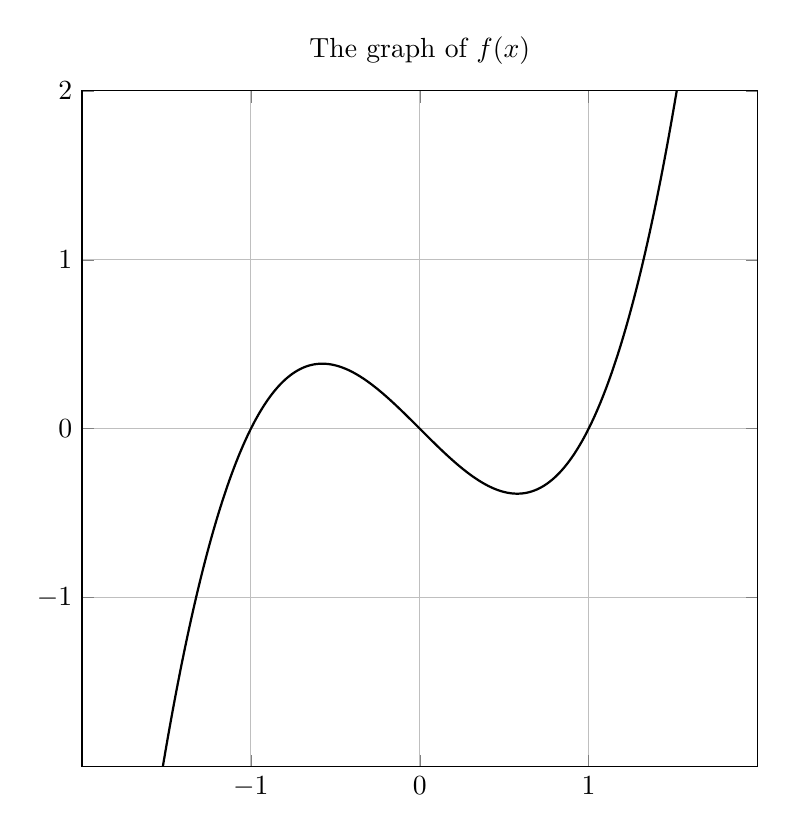
\begin{tikzpicture}
      \begin{axis}[width=4in, height=4in, smooth, samples=1000, grid=major, ymin=-2,ymax=2, xmin=-2, xmax=2, axis equal, xtick={-1,0,1}, ytick={-1,0,1,2},
        title={The graph of \(f(x)\)}
        ]
        \addplot[thick, black] {x^3 - x};
        % \node[right] (axis cs:1.5,1) {\footnotesize \(f'(x)\)};
      \end{axis}
    \end{tikzpicture}  

    \begin{tikzpicture}
      \begin{axis}[width=4in, height=4in, smooth, samples=1000, grid=major, ymin=-1.5,ymax=2.5, xmin=-2, xmax=2, axis equal, xtick={-1,0,1}, ytick={-1,0,1,2},
        title={The graph of \(f'(x)\)}
        ]
        % \addplot[thick, black] {3*x^2 - 1};
      \end{axis}
    \end{tikzpicture}  
  \end{center}
\end{example}

\clearpage

\section{Continuity and Non-differentiability}

\begin{mdframed}[style=withref]
  \textbf{Theorem}. If \(f\) is {differentiable} at \(a\), then \(f\) is {continuous} at \(a\).

  \textbook{\stewart{157}{\fbox{4} Theorem}}
\end{mdframed}

There are a few ways that a functions can fail to be differentiable.
\begin{enumerate}[label=(\alph*)]
  \item If a function is not continuous \(a\), then it is not differentiable at \(a\).

  \item If a function has a ``corner'' or a ``kink'', then it is not differentiable. 

  \item If a function \(f\) has a vertical tangent line at a point \((a,f(a))\), then it is also not differentiable.
\end{enumerate}

\bigskip
\begin{example}
  Explain (using one of the reasons above) why the following functions are not differentiable.

  \begin{enumerate}
    \item \(g_{1}(x) = \frac{x - 1}{x}\). \vfill
    \item \(g_{2}(x) = \begin{cases} 1 &\text{if } x \ge 0 \\ 0 &\text{if } x < 0 \end{cases}\). \vfill
    \item \(g_{3}(x) = x^{1/3}\). See its graph below.

      \begin{tikzpicture}[yscale=2, xscale=1.5]
        \draw[domain=-1:1] plot[samples=1000, smooth] ( {\x}, {\x^(1/3)} );
        \node[below] at (1,1) {\footnotesize \(x^{1/3}\)};
        \draw[thin, dotted] (-1,-1) grid (1,1);
        \node[left] at (-1, 1) {\footnotesize \(1\)};
        \node[left] at (-1, 0) {\footnotesize \(0\)};
        \node[left] at (-1,-1) {\footnotesize \(-1\)};

        \node[below] at ( 1,-1) {\footnotesize \(1\)};
        \node[below] at ( 0,-1) {\footnotesize \(0\)};
        \node[below] at (-1,-1) {\footnotesize \(-1\)};
      \end{tikzpicture}
    \item \(g_{4}(x) = |x|\).  \vfill
  \end{enumerate}
\end{example}

% \clearpage
% \section{Using information from \(f'(x)\)}
%
% \begin{example}
%   The velocity function \(g'(x)\) is given below. Sketch the displacement function \(g(x)\). Assume \(g(x)\) passes through the origin.
%
%   \begin{tikzpicture}
%     \begin{axis}[width=4in, height=4in, smooth, samples=1000, grid=major, ymin=-2,ymax=2, xmin=-3, xmax=3, axis equal, xtick={-2,-1,0,1,2}, ytick={-2,-1,0,1,2}, yticklabels={\phantom{-2},0,\phantom{-1},},
%       title={Displacement function \(g(x)\)}
%       ]
%       % \addplot[thick, black] {ln(4*x^2 + 1)/4 - 1};
%       \addplot coordinates { (0,-1) };
%     \end{axis}
%   \end{tikzpicture}  
%
%   \begin{tikzpicture}
%     \begin{axis}[width=4in, height=4in, smooth, samples=1000, grid=major, ymin=-2,ymax=2, xmin=-3, xmax=3, axis equal, xtick={-2,-1,0,1,2}, ytick={-2,-1,0,1,2},
%       title={Velocity function \(g'(x)\)}
%       ]
%       \addplot[thick, black] {rad(atan(x*2))};
%     \end{axis}
%   \end{tikzpicture}  
% \end{example}

\clearpage

Prove that if \(f\) is differentiable at \(a\), then \(f\) is continuous at \(a\).

Observation: \(\lim_{x \to a} f(x) = f(a)\) is equivalent to \(\lim_{x \to a} (f(x) - f(a)) = 0\).

\clearpage
\section{Selected questions from quiz 1}
\emph{True or false?} Suppose \(\lim_{x \to 1}f(x) = 0\) and \(\lim_{x \to 1}g(x) = 0\), then \(\lim_{x \to 1} \frac{f(x)}{g(x)}\) does not exist.
\vfill


If \(f\) is continuous at \(5\) and \(f(5) = 1\) and \(f(1) = 2\), then 
\vspace{1em}

\[
  \lim_{x \to 1} \phantom{x} f( \phantom{x} 4x^{2} + 1 \phantom{x}) = \phantom{MMMMMMMMMMMMMMMMMMMMMMM}
\]
\vspace{1in}


\emph{True or false?} If \(|f|\) is continuous at \(c\), then \(f\) is continuous at \(c\). 

\begin{tikzpicture}
  \begin{axis}[height=1.5in, width=2in, smooth, samples=100, ymin=-1, ymax=1, axis lines=middle, xticklabels={,,}, yticklabels={,,}, enlargelimits=true]
    \addplot[teal] coordinates { (0,1/2) (1,1/2) };
    \draw[teal, fill=white] (axis cs:1,1/2) circle (2pt);
    \fill[magenta] (axis cs:1,-1/2) circle (2pt);
    \addplot[magenta] coordinates { (1,-1/2) (2,-1/2) };

    \node[below right] at (axis cs:0,0) {\footnotesize \(f(x)\)}; 
  \end{axis}
\end{tikzpicture}
\quad
\begin{tikzpicture}
  \begin{axis}[height=1.5in, width=2in, smooth, samples=100, ymin=-1, ymax=1, axis lines=middle, xticklabels={,,}, yticklabels={,,}, enlargelimits=true]
    \addplot[teal] coordinates { (0,1/2) (1,1/2) };
    % \draw[teal, fill=white] (axis cs:1,1/2) circle (1pt);
    \fill[magenta] (axis cs:1,1/2) circle (2pt);
    \addplot[magenta] coordinates { (1,1/2) (2,1/2) };
    \node[below right] at (axis cs:0,0) {\footnotesize \(|f(x)|\)}; 
  \end{axis}
\end{tikzpicture}
\vfill
\clearpage

\end{document}
